\documentclass[12pt]{article}

\usepackage[utf8]{inputenc}
\usepackage[french]{babel}
\usepackage[margin=1in,headheight=13.6pt]{geometry}
\usepackage{amsmath}
\usepackage{amssymb}
\usepackage{graphicx}
\usepackage{caption}
\usepackage{subcaption}
\usepackage{float}
\usepackage{fancyhdr}

\pagestyle{fancy}
\fancyhf{}
\rhead{Team ADFTZ}
\lhead{Pattern Recognition}
\cfoot{\thepage}

\begin{document}
\title{Final Report}
\author{David Bücher, Timo Bürk, Félicien Hêche, Aleksandar Lazic, Zakhar Tymchenko }
\date{24.05.2020}
\maketitle


\section*{General Organization}
In our team, we organized our work as follows.
\newline When we got the first instructions for the assignment, we waited a week before we made the first Discord meeting. It was really helpful to really understand what we should do and to start thinking about the implementation. It was also a way to catch up with the theory if something was not clear. Then, we discussed our different point of view until we were in agreement on the implementation. Finally, we tried to divide the work as equally as possible between the different team members.
\newline We decided not to use a project management tool to organize our work, but we could have used something like Trello to clearly separate each member's tasks with the current status. Such tools are really useful in big projects as they give a better overview of the whole project (tasks to do, tasks done, ...)
\newline Then, each member worked alone on the assigned part. We also used a WhatsApp group for small communications, to keep in touch during the week. It was helpful to get a quick answer from the team about some details (what should be the output of a certain function, what do you think about the README, ...)
\newline  To be more precise, we could say that for the task 2a to 2d, a single person was assigned to the task. Indeed, since it was not too much work to do, we thought it could be more complicated if many people worked on it. But, the important points like the architecture or the general implementations were discussed on the Discord meeting. You'll find a more detailed description in the next section for each specific task.
\section*{Tasks}
In this section we'll talk about individual tasks we have worked on. Only Ex3 and Ex5 will be given more in-depth descriptions, since other had their own respective reports.
\subsection*{2a SVM}
In the first task we needed to use a support vector machine (SVM) to solve the MNIST dataset. Since we could choose any library we wanted, we used the sklearn library. Note, that we submitted two implementations of this task (version v1 and v2 on github). We had some misunderstandings about who should do the task and so, two people implemented it. But since, it seems to be a good work in both cases, we decided to put the two versions on github. Note that with this approach we were able to get an accuracy of 97,24\% on the validation set.
\subsection*{2b MLP}
Then, we implemented a Multiple Layer Perceptron (MLP) to solve the MNIST dataset. To build our MLP, we used the MLPClassifier class provided by sklearn, and for the grid search, we used the function GridSearchCV also provided by sklearn. With these different approach, we were able to get an accuracy of about 97.5\% on the validation set.
\subsection*{2c CNN}
In the task 2c, we needed to make a Convolutional Neural Network (CNN) to solve the MNIST dataset. To do it, we use the PyTorch library. The model we used was composed of three convolutional layers (always followed by the LeakyReLu activation function). And for the classification head, we used a simple linear layer.
With this model, we get a 98,5\% accuracy on the validation set.
\subsection*{2d MLP and CNN on permutated MNIST}
After that, in the task 2d, we had to train and test our MLP and CNN model on a permutated MNIST dataset. We expected that the MLP will have about the same accuracy that the model train  the real MNIST dataset. And for our CNN, we thought it will have a lower accuracy that on MNIST.
\newline We observe an accuracy of 94,6\% for the MLP (vs 97,5\% on the normal MNIST) and for the CNN, we get an accuracy of 93\% (vs 98.5\%). So, as expected the MLP is less sensitive than the CNN to the original positions, but there is less differences than we thought.

\subsection*{3 Keyword Spotting with Dynamic Time Wrapping}

Since this project was bigger than the previous tasks, we split it in the following parts:
\begin{enumerate}
\item[•]Features Extraction Implementation.
\item[•]Dynamic Time Wrapping Implementation.
\item[•]Evaluation.
\end{enumerate}
Then, each task were done by a different person with a defined deadline, to be sure that we would be able to submit the project in time.

\subsubsection*{Implementation}

We used and SVG library, PIL, skimage and cv2 for image processing - to extract the words from the document, put them through a black-and-white filter and save them for further usage.

Then we processed the dataset for further usage. After the image was "simplified" we applied a cut-off of fully white rows and columns from all sides (more about this later) and resized the image to 100px by 100px. Then we performed a feature extraction for DWT. The feature set is relatively simplistic - ratio of black pixels, counters of black and white pixels, earliest/latest black pixels.

Afterwards we do a standard DWT using a cost matrix where we limit our search path using a Sakoe-Chiba band with a window of $w = 0.3$. This gave an acceptable performance as well as precision.

To match words to each other using their labels, we perform a simplification of words, which can be found in our utilities collection file. We mostly remove punctuation. This has overall increased the performance of the algorithm.

\subsubsection*{Cutting the image}

The main idea was to rid the image of useless information, notable lines and columns from the extremes that don't contain a single black pixel. Otherwise DWT will partially measure the dissimilarity of the polygon that cuts the word, which we wanted to exclude from the equation.

We search from each side of the image rows (or columns) which are completly white, and then we just remove them from the image.

\begin{figure}
     \centering
     \begin{subfigure}[b]{0.3\textwidth}
         \centering
         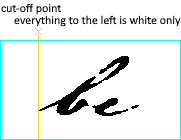
\includegraphics[scale=1.0]{figs/grey_nocut.png}
         \caption{Without the cut}
         \label{fig:grey_nocut}
     \end{subfigure}
     \begin{subfigure}[b]{0.3\textwidth}
         \centering
         
\includegraphics[scale=1.0]{figs/grey_cut.png}
         \caption{With the cut}
         \label{fig:grey_cut}
     \end{subfigure}
        \caption{Differences of black-and-white images before and after the cut.}
        \label{fig:orig_grey}
\end{figure}

Figure~\ref{fig:grey_nocut} shows the original image and how a cut-off line is determined from the left side (Cyan block denotes image borders.). If we repeat this process 4 times (left, right, top, bottom) we obtain the image in Figure Figure~\ref{fig:grey_cut}.

The process is performed before resizing and the difference is very noticeable. After resizing into 100x100 an uncut image Figure~\ref{fig:nocut_resize} shows that the biggest area that doesn't contain fully white rows/columns at the edges is only 56x62. This is 34.72\% of the area of the full picture.

Effectively there's a lot of information about the word that is lost and in the remaining 65.28\% of the image DWT will measure the similarity of the polygon used to cut the word out of the page. While in Figure~\ref{fig:cut_resize} the word takes up the whole image, nothing can be cut from the sides without losing the information about the word.

\begin{figure}
     \centering
     \begin{subfigure}[b]{0.3\textwidth}
         \centering
         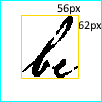
\includegraphics[scale=1.0]{figs/nocut_resize.png}
         \caption{Resized original}
         \label{fig:nocut_resize}
     \end{subfigure}
     \begin{subfigure}[b]{0.3\textwidth}
         \centering
         
\includegraphics[scale=1.0]{figs/cut_resize.png}
         \caption{Resized cut}
         \label{fig:cut_resize}
     \end{subfigure}
        \caption{Differences between resized versions of images.}
        \label{fig:resized}
\end{figure}

Figure~\ref{fig:cutoff_ex} shows the ranking of dissimilarities of the word "the", ordered ascending, i.e. most similar matches on top. Left window is an uncut version, right window is the cut version. It's a screenshot of an editor with search that highlights the search results on the scroll bar where we search for the exact (minus capitalization) matches.

Notice how distribution of matches shifts up on the right side of the editor where we perform an image cut-off. The one of the left has a lot of matches in the upper part, but everything below the first 40\% is distributed almost uniform until the very end. While on the right side, upper 30\% are much more packed and lower 30\% don't contain almost any matches at all.

\begin{figure}
    \centering
    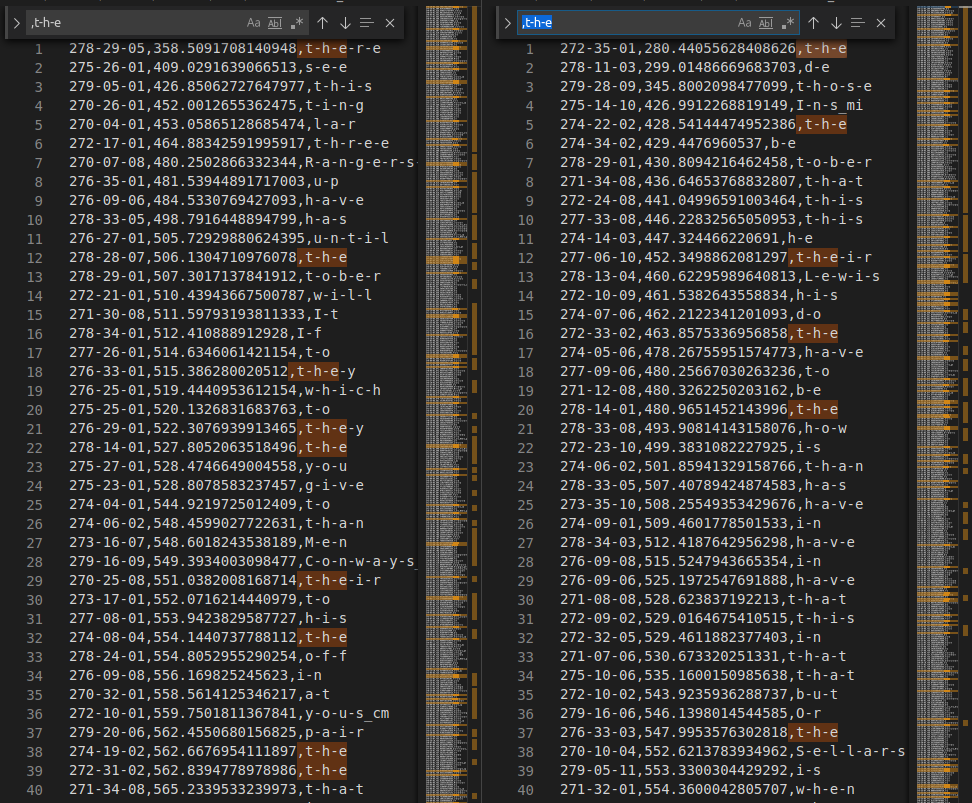
\includegraphics[scale=0.45]{figs/cutoff-ex.png}
    \caption{DWT rankings of the word "the". Cut version is on the right.}
    \label{fig:cutoff_ex}
\end{figure}

\subsubsection*{Evaluation}

For evaluation we plotted precision-recall curves which can be found in the repository. Additional curves (for keywords outside of 'keywords.txt') can be plotted too, the program can be ran to include them all, see README of task 3.

\subsection*{5 Molecules}
For the last task, since we have already implemented a Dynamic Time Wrapping in the previous task, we choose to work on the Molecules task. We split it in two different tasks. One person did the parsing and a person implemented the Graph Edit Distance.

\subsubsection*{Implementation}

Since the data set is of reasonable small size, and the data structure relatively complex,
we use a simple "homemade" KNN implementation.

Our GED is technically not a "full" graph edit distance as we used a shortcut for the Edge Assignment Cost. The intuition is that the structure of molecules is heavily influenced by the nature of the atoms. For example: carbon tends to have between 2 and 4 neighbors while hydrogen only one.

This means we cab do kind of a partial editing distances where we assign a cost for changing the nodes symbols, and a little adjustment based on the difference of edges. For nodes $n_1$ and $n_2$ we compute it as $|$deg$(n_1) - $deg$(n_2)|$. As this is significantly more simple to implement, and produces good results, we consider this approach a success.

\subsubsection*{Parameter optimization and evaluation}

To optimize parameters we split the train set in two subsets, and test the accuracy for given combination of parameters (Cn, Ce, K).
The results can be seen in the table in Table~\ref{fig:res_table}. We encountered multiple instances of $100\%$ accuracy. Since this can be a sign of overfitting, we decided to select
our final parameters based on the second best accuracy observed during this phase, which is $99.40\%$. Of the available candidates with this accuracy we selected one at random: $C_n = 1, C_e = 1, K = 3$.

\begin{table}[h]
\centering
\begin{tabular}{|c|c|c|c|c|}
& K = 1 & K = 3 & K = 5 & K = 7\\
\hline
$C_n = 1, C_e = 0$ & $91.02\%$ & $\textbf{100.0\%}$ & $\textbf{100.0\%}$ & $98.20\%$\\
$C_n = 1, C_e = 1$ & $92.22\%$ & $99.40\%$ & $99.40\%$ & $\textbf{100.0\%}$\\
$C_n = 1, C_e = 2$ & $88.62\%$ & $98.80\%$ & $99.40\%$ & $\textbf{100.0\%}$\\
$C_n = 1, C_e = 3$ & $88.62\%$ & $98.80\%$ & $\textbf{100.0\%}$ & $\textbf{100.0\%}$\\
\hline
$C_n = 2, C_e = 0$ & $91.02\%$ & $\textbf{100.0\%}$ & $\textbf{100.0\%}$ & $98.20\%$\\
$C_n = 2, C_e = 1$ & $94.01\%$ & $99.40\%$ & $99.40\%$ & $\textbf{100.0\%}$\\
$C_n = 2, C_e = 2$ & $92.22\%$ & $99.40\%$ & $99.40\%$ & $\textbf{100.0\%}$\\
$C_n = 2, C_e = 3$ & $91.01\%$ & $99.40\%$ & $\textbf{100.0\%}$ & $\textbf{100.0\%}$\\
\hline
$C_n = 3, C_e = 0$ & $91.02\%$ & $\textbf{100.0\%}$ & $\textbf{100.0\%}$ & $98.20\%$\\
$C_n = 3, C_e = 1$ & $95.81\%$ & $99.40\%$ & $\textbf{100.0\%}$ & $\textbf{100.0\%}$\\
$C_n = 3, C_e = 2$ & $94.01\%$ & $99.40\%$ & $99.40\%$ & $\textbf{100.0\%}$\\
$C_n = 3, C_e = 3$ & $92.22\%$ & $99.40\%$ & $99.40\%$ & $\textbf{100.0\%}$\\
\end{tabular}\\
\caption{Parameter tuning table}
\label{fig:res_table}
\end{table}

With our final chosen parameters we got a good result, the accuracy on validation set was $99.20\%$.

\section*{General Thoughts}
In general, we think that our team worked quite well. We did not have any big issues. Of course, all was not perfect and we could had improved some things. For example, at the beginning, we had some communications problems. It was not really clear what each member should do. For this reason, we have two versions of the task 2b. But after this small misunderstanding, all worked fine and we are quite satisfied about the submitted project.
\newline Concerning the project itself, it was really nice that we were free to use either existing libraries or to implement the different algorithms ourselves. Although it is often unnecessary to re-implement existing libraries, it helps understanding the algorithm more in depth.

\end{document}
